\section*{Introduction}


\begin{frame}
    \frametitle{Introduction}
    \begin{itemize}
        \item How do vaccines work? What are the different types of vaccines?
        \item To what extent do mRNA vaccines represent a breakthrough?
        \item How do societies use and adapt to the development of vaccine?
    \end{itemize}

    \begin{figure}
        \centering
        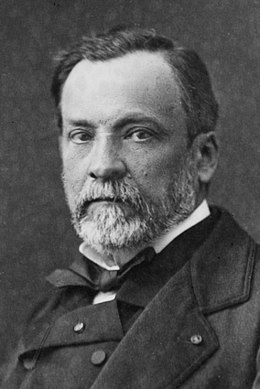
\includegraphics[width=0.3\textwidth]{imgs/paster.jpg}
        \caption{Dr. Pasteur}
        \label{fig:responses4}
    \end{figure}

\end{frame}

\section{A brief history of vaccines}
\subsection{A quick look on immunology}


\begin{frame}
    \frametitle{The immune system}
\begin{figure}
    \centering
    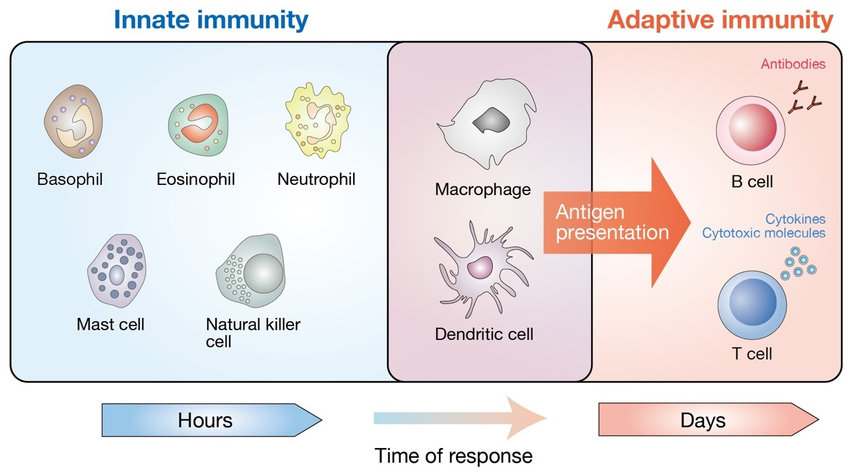
\includegraphics[width=0.8\textwidth]{imgs/ImmunityCells.png}
    \caption{Main cells of the immune system \autocite{yamauchiHippoPathwayMammalian2019}}
    \label{fig:responses3}
\end{figure}
\end{frame}

\begin{frame}
    \frametitle{How to communicate?}
\begin{figure}
    \centering
    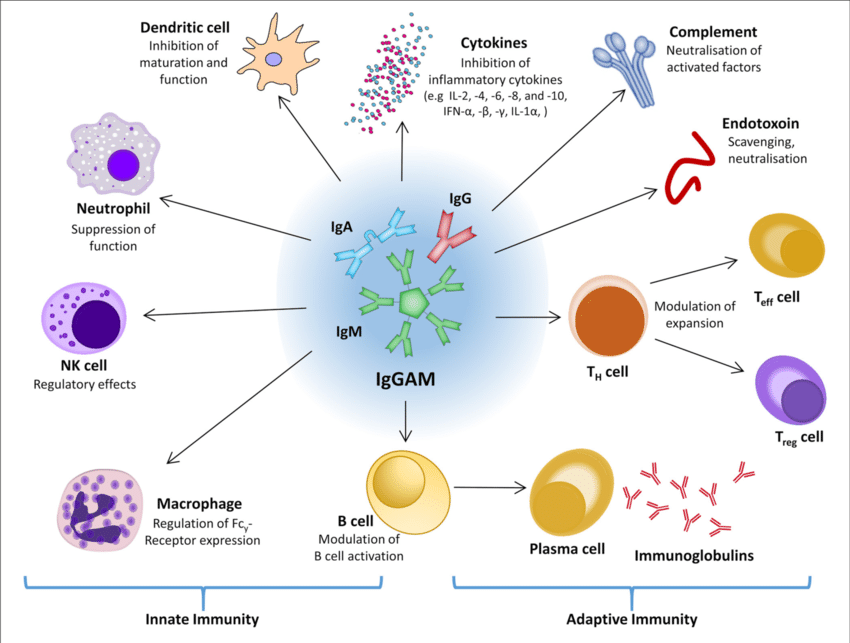
\includegraphics[width=0.7\textwidth]{imgs/Communication.png}
    \caption{Major roles of each cells \autocite{jarczakSepsisPathophysiologyTherapeutic2021}}
    \label{fig:responses10}
\end{figure}
\end{frame}

\begin{frame}
    \frametitle{The immune memory}
\begin{figure}
    \centering
    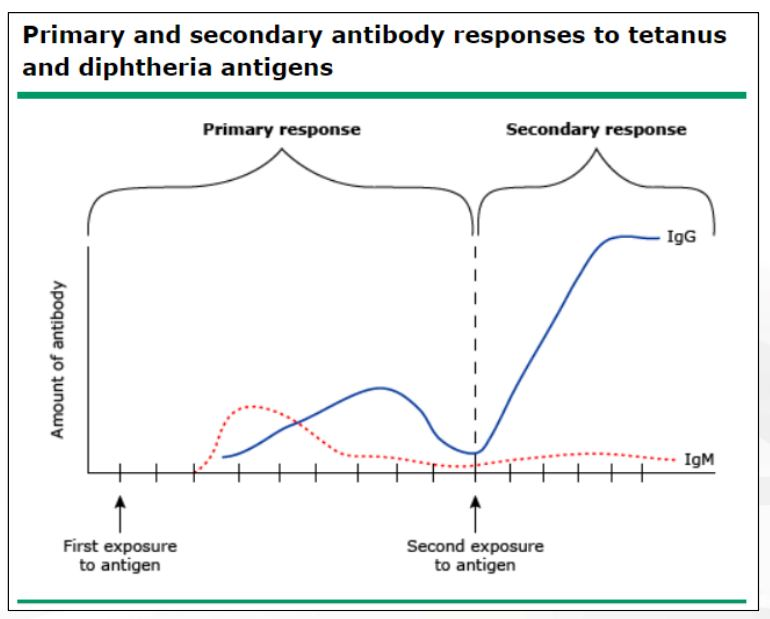
\includegraphics[width=0.7\textwidth]{imgs/PrimarySecondaryResponses.JPG}
    \caption{Primary and secondary responses to specific antigens \autocite{pinkComparisonImmunityGeneral}}
    \label{fig:responses12}
\end{figure}
\end{frame}

% PAMPS et DAMPS
%cytokines

\subsection{The different generations of vaccines}

\begin{frame}
    \frametitle{Three main approaches through time}
    \begin{figure}
        \centering
        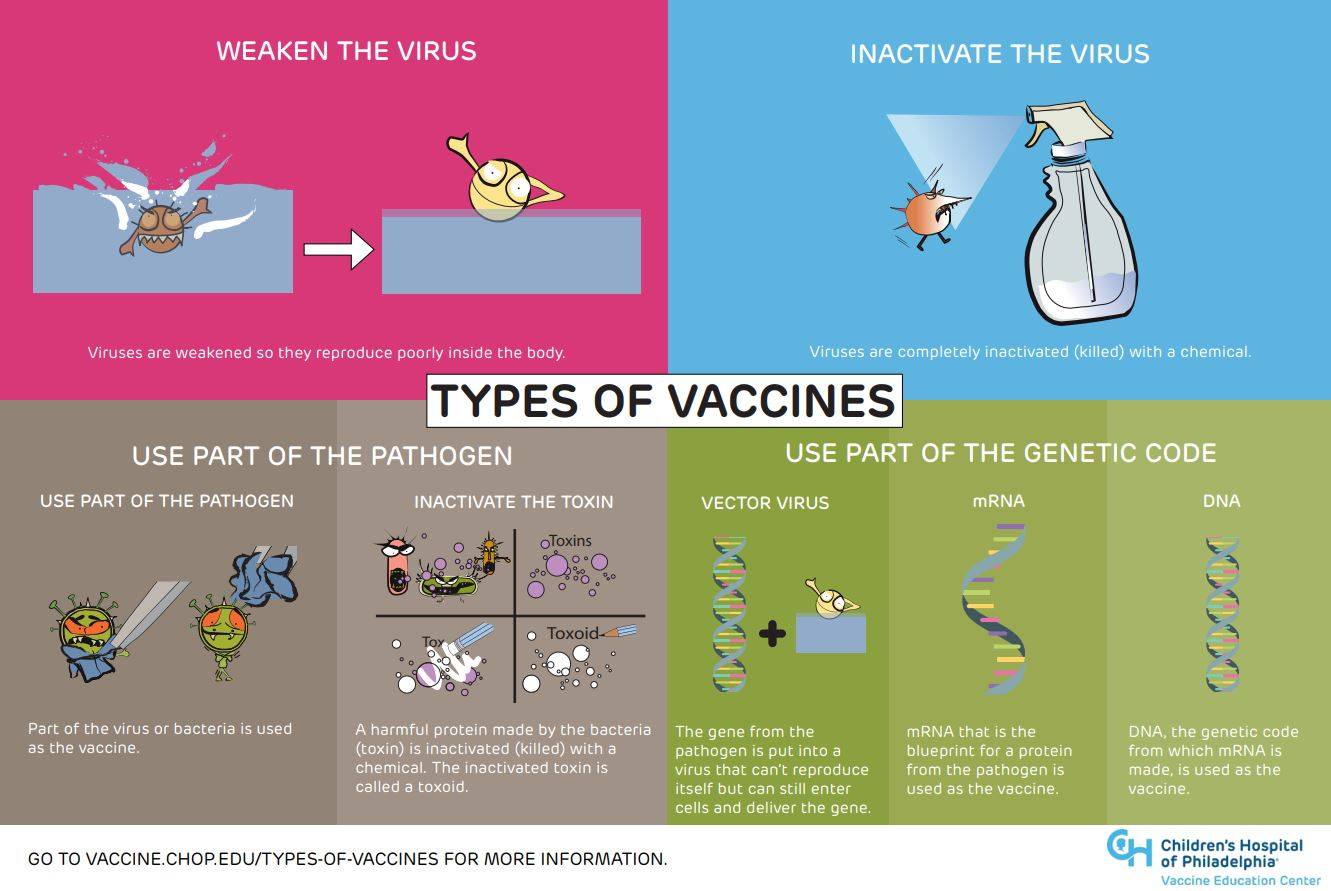
\includegraphics[width=0.8\textwidth]{imgs/VaccineGeneration.JPG}
        \caption{The different types of vaccines \autocite{philadelphiaMakingVaccinesHow2014}}
        \label{fig:responses2}
    \end{figure}
\end{frame}

\section{mRNA vaccines: a promising technology}
\subsection{Principle}

\begin{frame}{A new way of immunization}
    
    \begin{figure}
        \centering
        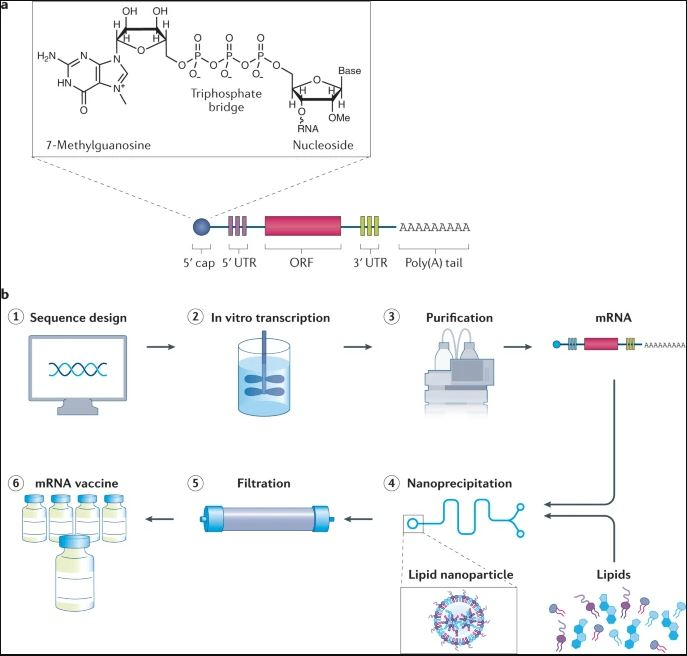
\includegraphics[width=0.5\textwidth]{imgs/mRNA_Vaccine.JPG}
        \caption{Process to produce mRNA vaccines \autocite{MRNAVaccinesInfectious}}
        \label{fig:mRNAvac}
    \end{figure}
    
\end{frame}

\subsection{Development}

\begin{frame}{Building a mRNA vaccine}
    
    \begin{figure}
        \centering
        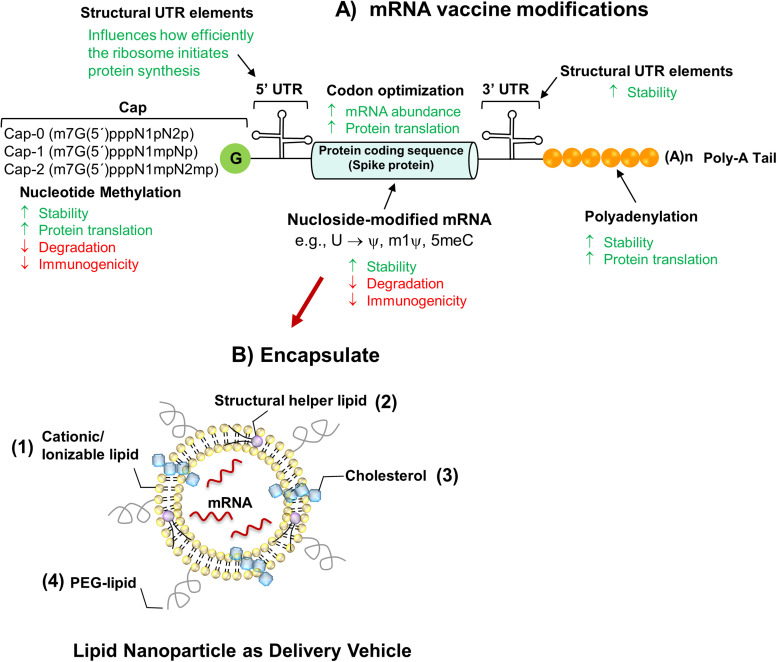
\includegraphics[width=0.6\textwidth]{imgs/RNA2.jpg}
        \caption{Choosing the right mRNA \autocite{granados-riveronEngineeringCurrentNucleosidemodified2021}}
        \label{fig:mRNAvac2}
    \end{figure}
    
\end{frame}

\begin{frame}{Two types of mRNA}
\begin{figure}
    \centering
    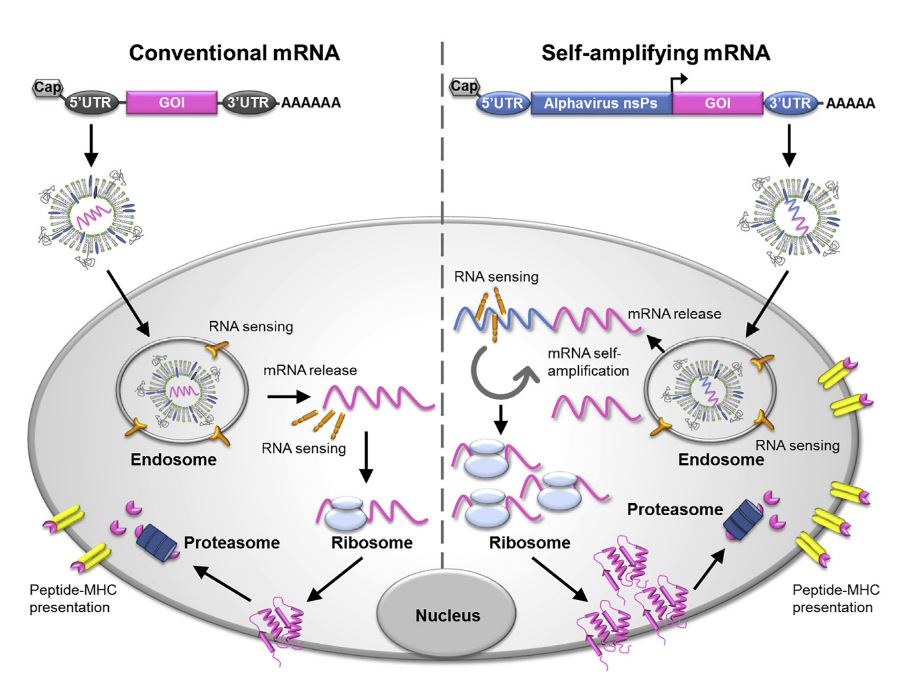
\includegraphics[width=0.65\textwidth]{imgs/mRNA_action.JPG}
    \caption{Comparison between conventional and self-amplifying mRNA \autocite{MRNATransformativeTechnology}}
    \label{fig:mRNAtypes}
\end{figure}
\end{frame}


\subsection{Evolution or revolution?}


\begin{frame}
    \frametitle{The COVID-19 case study: vaccine development}
    \begin{figure}
        \centering
        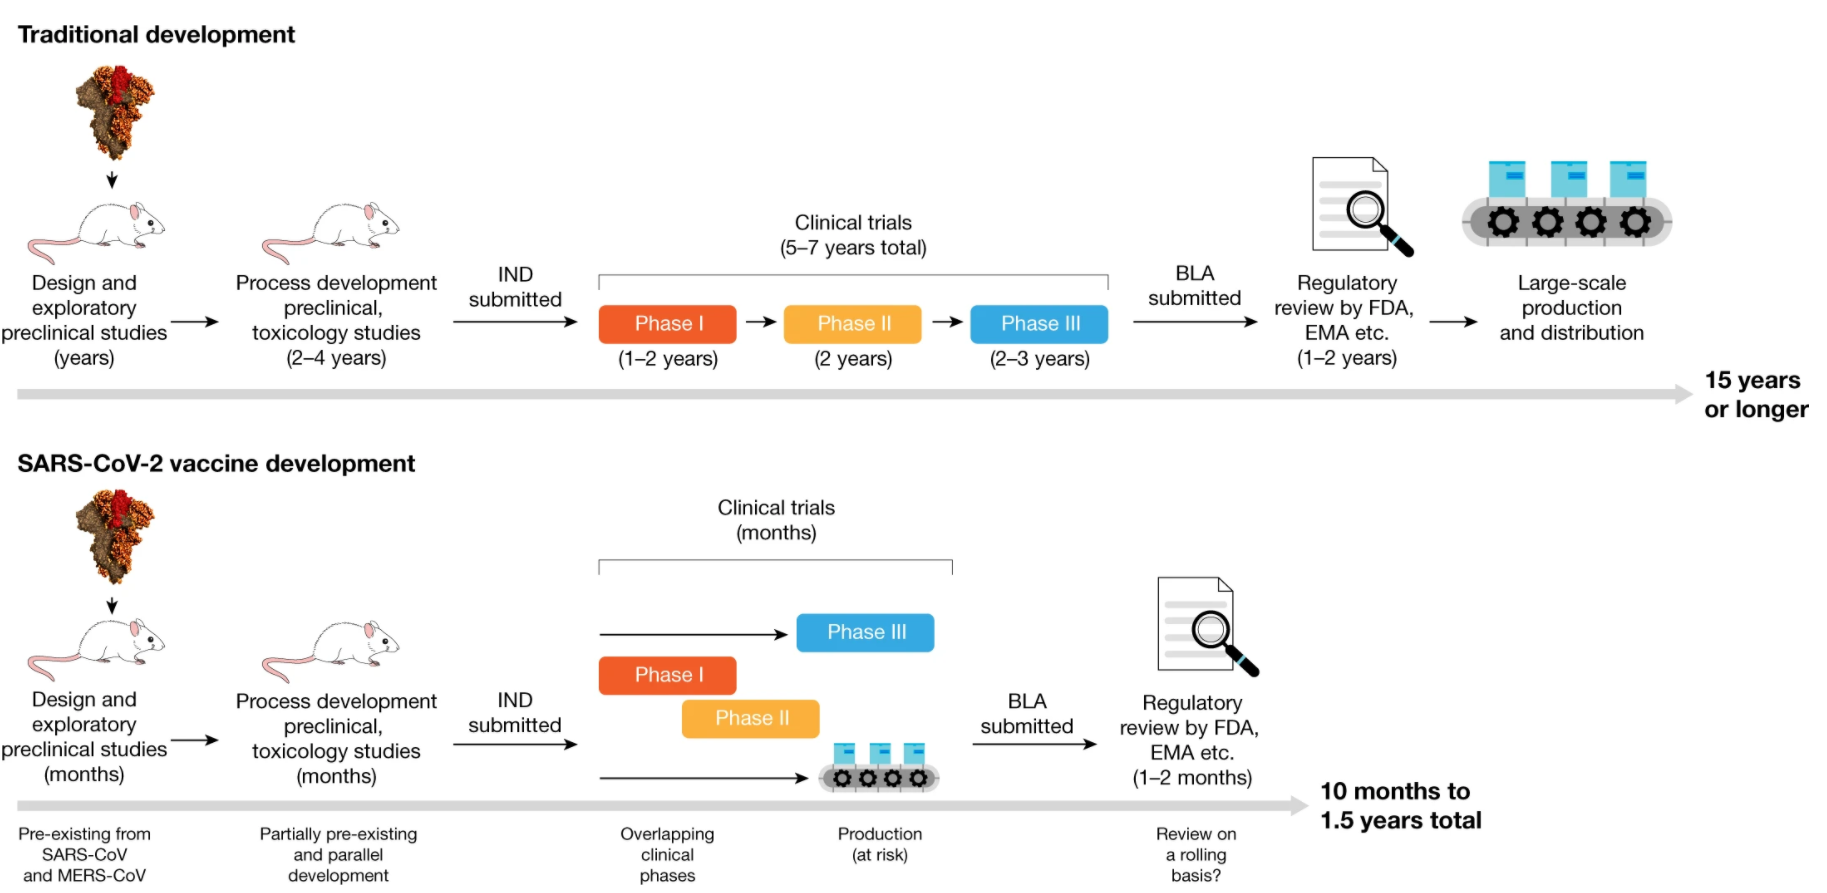
\includegraphics[width=0.9\textwidth]{imgs/CovidDev.png}
        \caption{Comparison of vaccine developments \autocite{krammerSARSCoV2VaccinesDevelopment2020}}
        \label{fig:responses5}
    \end{figure}
\end{frame}

\begin{frame}{What is possible thanks to mRNA?}
    Major advances:
    \begin{itemize}
        \item Computer support
        \item On demand vaccine, more investments
        \item Cancer treatment %https://www.cancer.gov/news-events/cancer-currents-blog/2022/mrna-vaccines-to-treat-cancer
        \item Therapeutic application
    \end{itemize}
    Some obstacles:
    \begin{itemize}
        \item Preservation
        \item Public acceptance (and scientific acceptance)
    \end{itemize}
\end{frame}

\section{New stakes for vaccines in the 21\up{st} century}
\subsection{World inequalities}

\begin{frame}
    \frametitle{The COVID-19 case study: vaccine inequalities}
    \begin{figure}
        \centering
        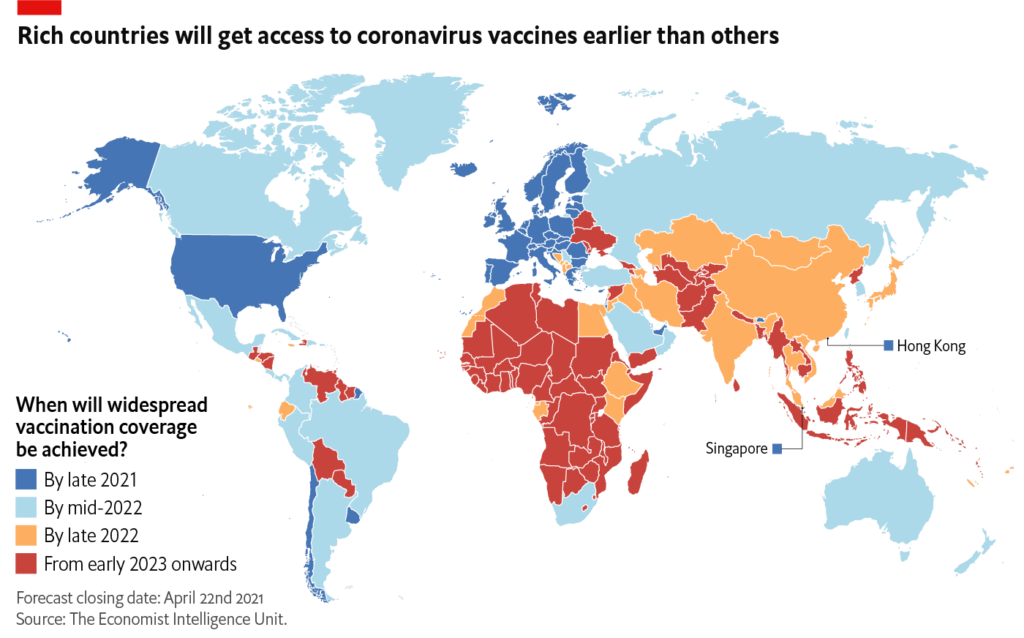
\includegraphics[width=0.8\textwidth]{imgs/Inequalities.png}
        \caption{COVID-19 vaccine deliveries (source \emph{The Economist})}
        \label{fig:responses6}
    \end{figure}
\end{frame}

\subsection{Public policies}

% Global Vaccine Action Plan
% immunization agenda 2030

\begin{frame}
    \frametitle{Public health necessity}
    \begin{figure}
        \centering
        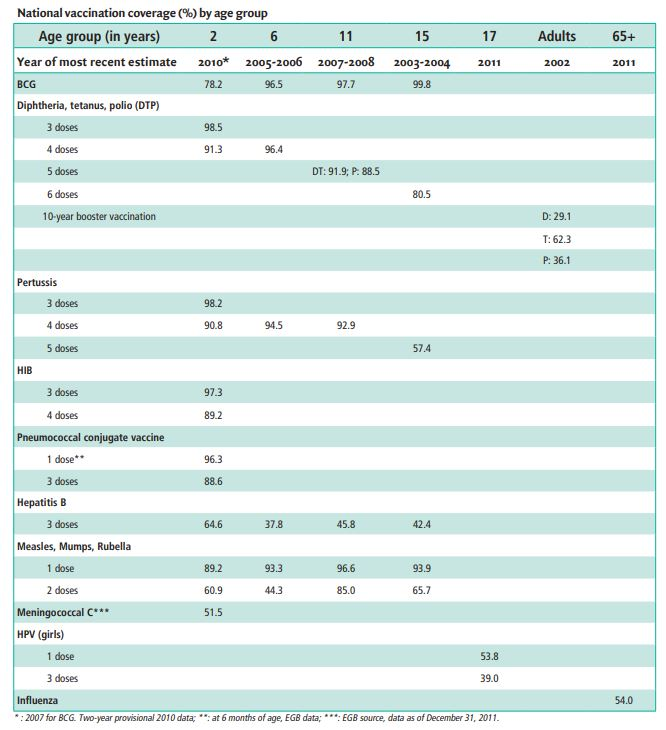
\includegraphics[width=0.5\textwidth]{imgs/VaccineSchedule.JPG}
        \caption{Vaccine schedule in France (Institut de veille sanitaire, InVS) \autocite{spfAssessmentVaccinationCoverage}}
        \label{fig:responses7}
    \end{figure}
\end{frame}
% Franco polio Spain 1950-1963

\begin{frame}
    \frametitle{Anti-vax: vaccine hesitancy}
    \begin{figure}
        \centering
        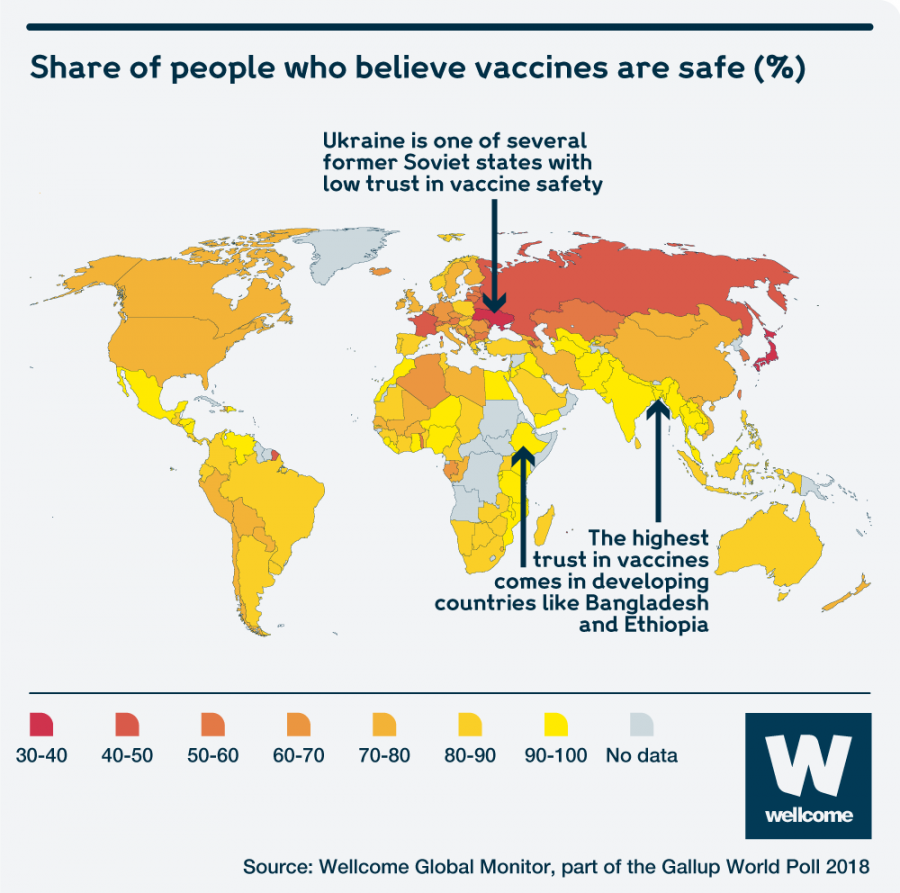
\includegraphics[width=0.5\textwidth]{imgs/VaccineHesitancy.png}
        \caption{Global survey about vaccine safety \autocite{SurveyRevealsEuropean}}
        \label{fig:responses8}
    \end{figure}
\end{frame}
% why lose faith : adverse effect, trust, fake news (alter DNA), bill gates (chip), conspiracy theories

\subsection{New perspectives for the future}

\begin{frame}
    \frametitle{The big picture}
    \begin{figure}
        \centering
        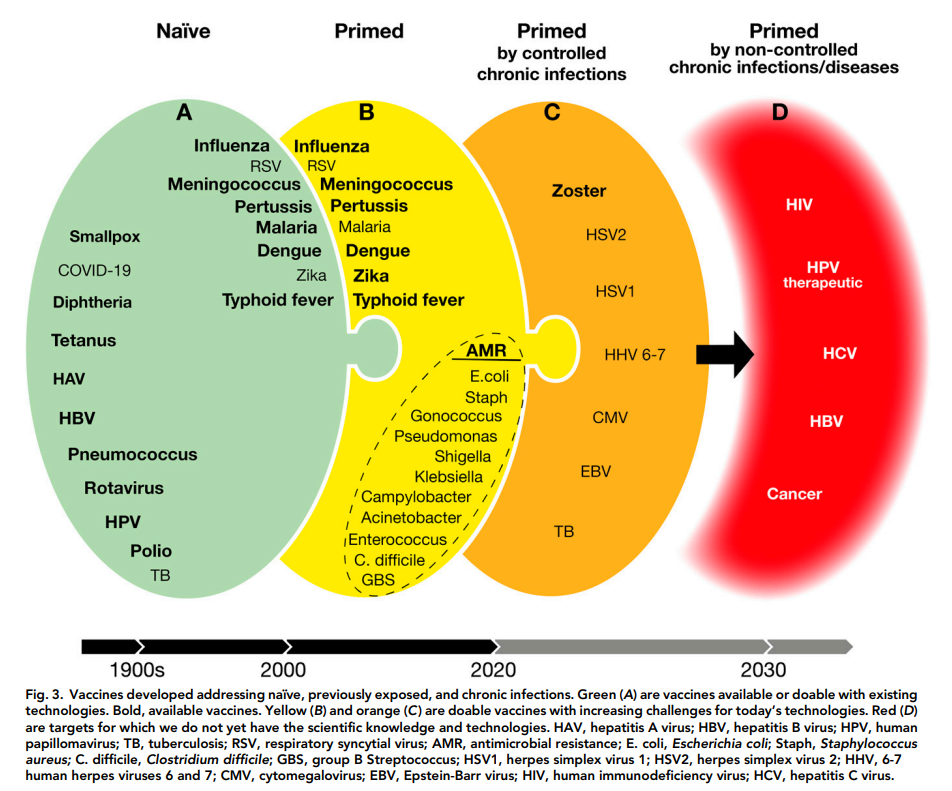
\includegraphics[width=0.65\textwidth]{imgs/vaccineEvolution.PNG}
        \caption{What to expect about vaccines? \autocite{rappuoliVaccinologyPostCOVID192021}}
        \label{fig:responses13}
    \end{figure}
\end{frame}
% why lose faith : adverse effect, trust, fake news (alter DNA), bill gates (chip), conspiracy theories





\section*{Conclusion}

\begin{frame}{Conclusion}
\begin{itemize}
    \item Active field of research since the eighteenth century
    \item At the crossroads of medicine, biology, chemistry and computer science
    \item 50 million future deaths averted from 2021-2030
    \item New challenges to face to continue vaccine development and avoid rejection
\end{itemize}
\begin{figure}
    \centering
    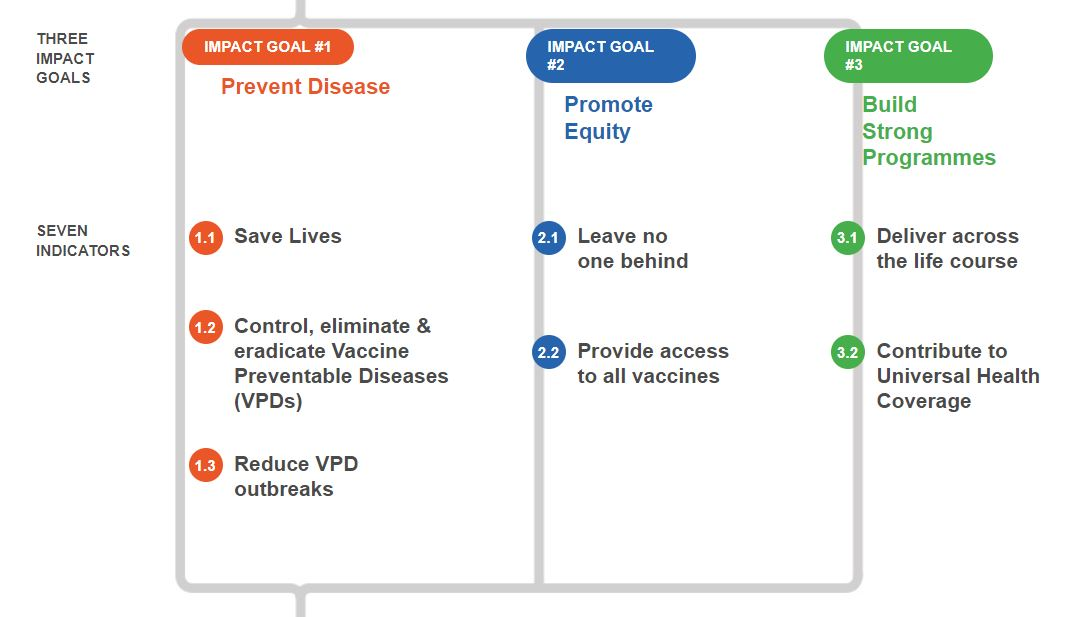
\includegraphics[width=0.5\textwidth]{imgs/Objectives.JPG}
    \caption{Immunization agenda 2030 (source WHO)}
    \label{fig:responses9}
\end{figure}
\end{frame}
% 10m

